\documentclass[a4paper]{scrreprt}

%% Language and font encodings
\usepackage[english]{babel}
\usepackage[utf8x]{inputenc}
\usepackage[T1]{fontenc}

%% Sets page size and margins
\usepackage[a4paper,top=3cm,bottom=2cm,left=3cm,right=3cm,marginparwidth=1.75cm]{geometry}

%% Useful packages
\usepackage{amsmath}
\usepackage{graphicx}
\usepackage[colorinlistoftodos]{todonotes}
\usepackage[colorlinks=true, allcolors=blue]{hyperref}

\title{Homeless}
\subtitle{"A game played from the perspective of a homeless person"}
\author{Andrusyak Bohdan, Gabl Sebastian, Huber Christian, Potzinger Dominic,\\Toller Maximilian and Voulgaridis Anastasios}
%\titlehead{\centering\includegraphics[width=6cm]{title_screen_mockup.png}}


\begin{document}
\maketitle

\null\vfill
\noindent
Game Design Document Template\\ 
Version v1.1, Nov 2016\\
Version v1.2, Dec 2017\\
Copyright 2017 - Johanna Pirker \#tugamedev\\
\newpage
\begin{abstract}
\textit{Homeless} is a game that is played from the perspective of a homeless person, who is trying to get through the day. It is inspired by survival games like "Don’t Starve" or "This War of Mine" and has similar features. The player has to manage living on the street, collecting food and finding shelter from rough weather. The game features a fixed camera angle in a 3D environment, with 2D character and object sprites. Players are able to interact with the environment, by clicking on objects and items, much like "Don’t Starve". Movement is handled by clicking on a spot in the world where the player wants to go. Game mechanics also include interaction with NPCs, both benevolent and malevolent. Players will encounter situations that require them to choose between multiple interactions that can affect NPCs positively or negatively while a Karma system keeps track of the players choices. Past decisions might then affect players later in the game.
\end{abstract}

\tableofcontents

% ______________________
% chapter Overview
% ______________________
\chapter{Overview}

%Main features and aspects of your game on a first page, describing story elements. -> "selling page", publisher should be able to decide after reading this single page whether to buy in or not 


\section{Main Concept}
Our main concept is to show how hard it is to be at societies bottom. Things which are natural for most of us can be a challenge for a homeless person. We want to show how hard it is to get enough to eat, a place to sleep or simply social interactions. Our game will at some stages seem hard or unfair. And in fact, that's the point. It depicts a life in poverty and shows the helplessness of people living in poverty. Sickness, death, hunger, crime and social proscription are the main aspects we want to address. We don't want players to simply collect and craft stuff and get a happy ending. What we want is to give players insight. What we want is to raise awareness for those in need of a life in dignity.

\section{Unique Selling Point}
%describe you unique selling point in one paragraph

\textit{Homeless} tells a different story. It's neither an epic, nor a fairy tale. It doesn't communicate glory, perfection or greatness. \textit{Homeless} is a story about a blind spot in our society. It grasps what is normal and twists it to a sad, cruel and fascinating perspective, creating unique settings, unexpected tools, and a merciless world located in the center of everything we take for granted. 


% ______________________
% chapter References
% ______________________

\chapter{References} 
%research on similar games, what are the core features, how does your game differ?\\
\textit{Homeless} is inspired by survival games like "Don't Starve" and "This War of Mine" and builds on similar concepts. While "Don't Starve" is mostly about the character $\leftrightarrow$ environment interaction and "This War of Mine" strongly emphasizes character $\leftrightarrow$ character interaction, we want to combine both of them and find a good middle ground. We also try to capture a similar atmosphere as "This War of Mine" where no decision is easily made and might introduce consequences that hinder or support the players further progress. We want the player to ponder his or her decisions and we want them to recognize that their decisions make differences.

\begin{figure}[h]
\centering
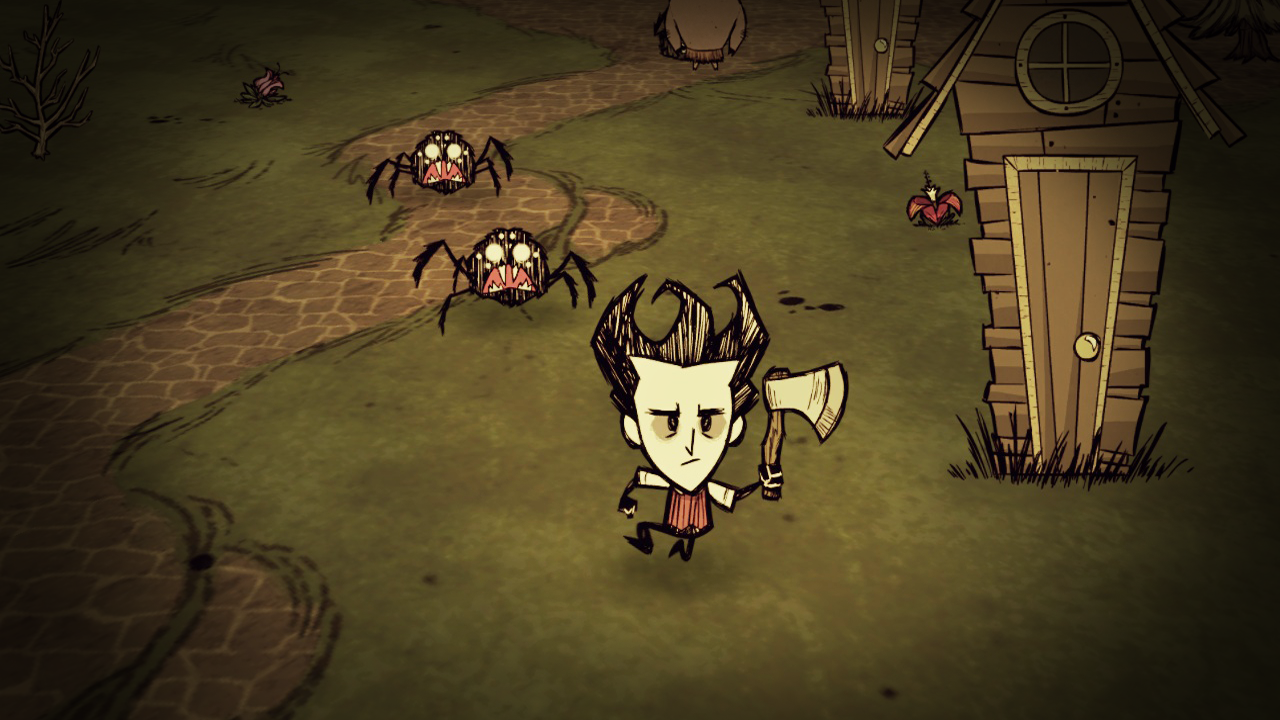
\includegraphics[width=0.8\textwidth]{dontstarve.png}
\caption{\label{fig:ds} Don't Starve}
\end{figure}

\begin{figure}[h]
\centering
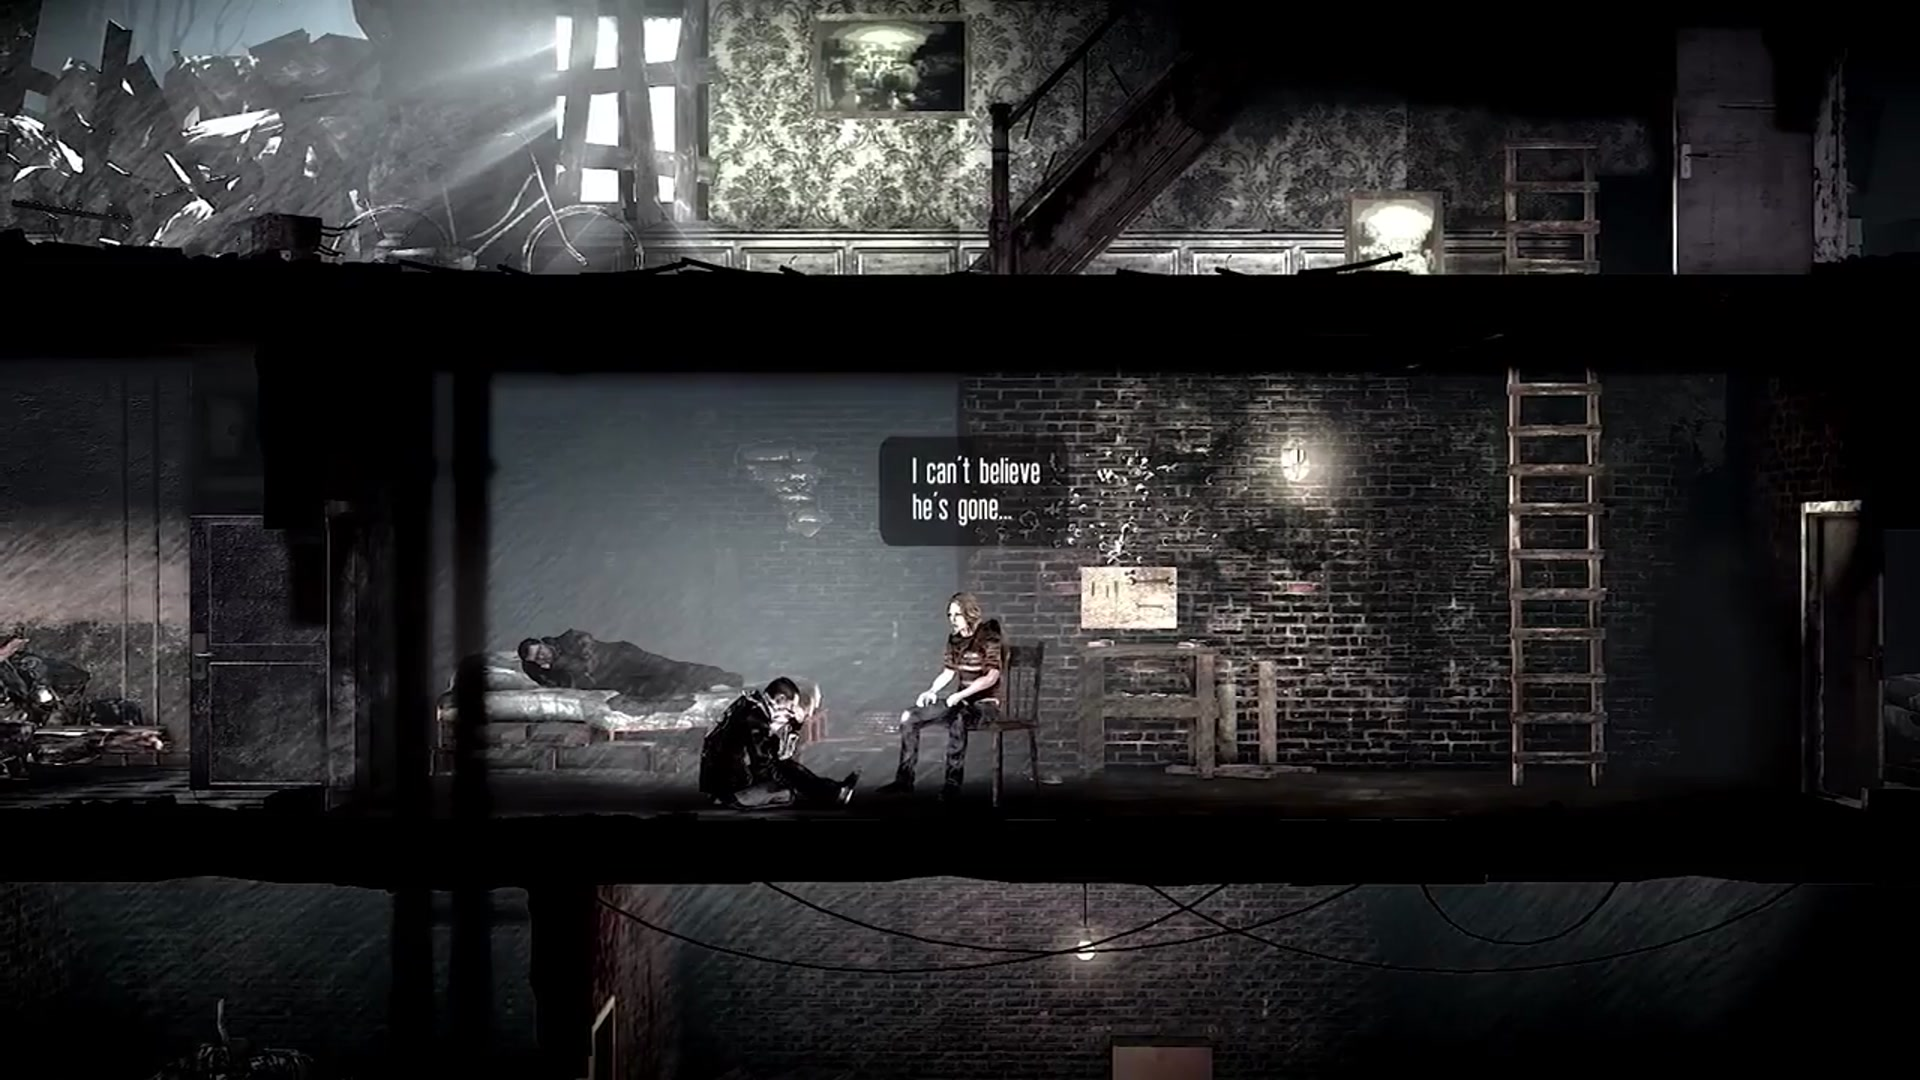
\includegraphics[width=0.8\textwidth]{TWoM.jpg}
\caption{\label{fig:twom} This War of Mine}
\end{figure}

% ______________________
% chapter Specification and Market Analysis 
% ______________________

\chapter{Specification}
%description of target group, platform, art style, who to attract of how to attract 

\section{Player(s) / Target-group}
We certainly want to reach as many people as possible to raise awareness, but due to the aspects our game addresses we are interested in people of age 16 or older. The age is chosen because our game will include violence and depressing content.\\
Apart from the age limit we want to reach men and women which are interested in playing a game which focuses on societal contents. People who like the story and general feel of "This War Of Mine" combined with the mechanics of "Don't Starve" will most certainly also like \textit{Homeless}.

\section{Genre}
\textit{Homeless} is an Open-World-Survival game.

\section{Art Style}
The game features a simplistic art style with 2D character and object sprites and a desaturated color scheme.

\begin{figure}[h]
\centering
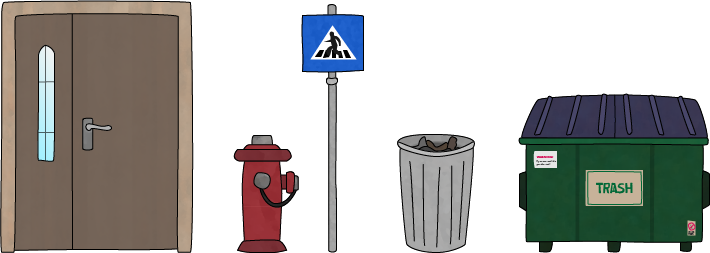
\includegraphics[width=1\textwidth]{artstyle.png}
\caption{\label{fig:art} Assortment of objects displaying the art style}
\end{figure}

\begin{figure}[h]
\centering
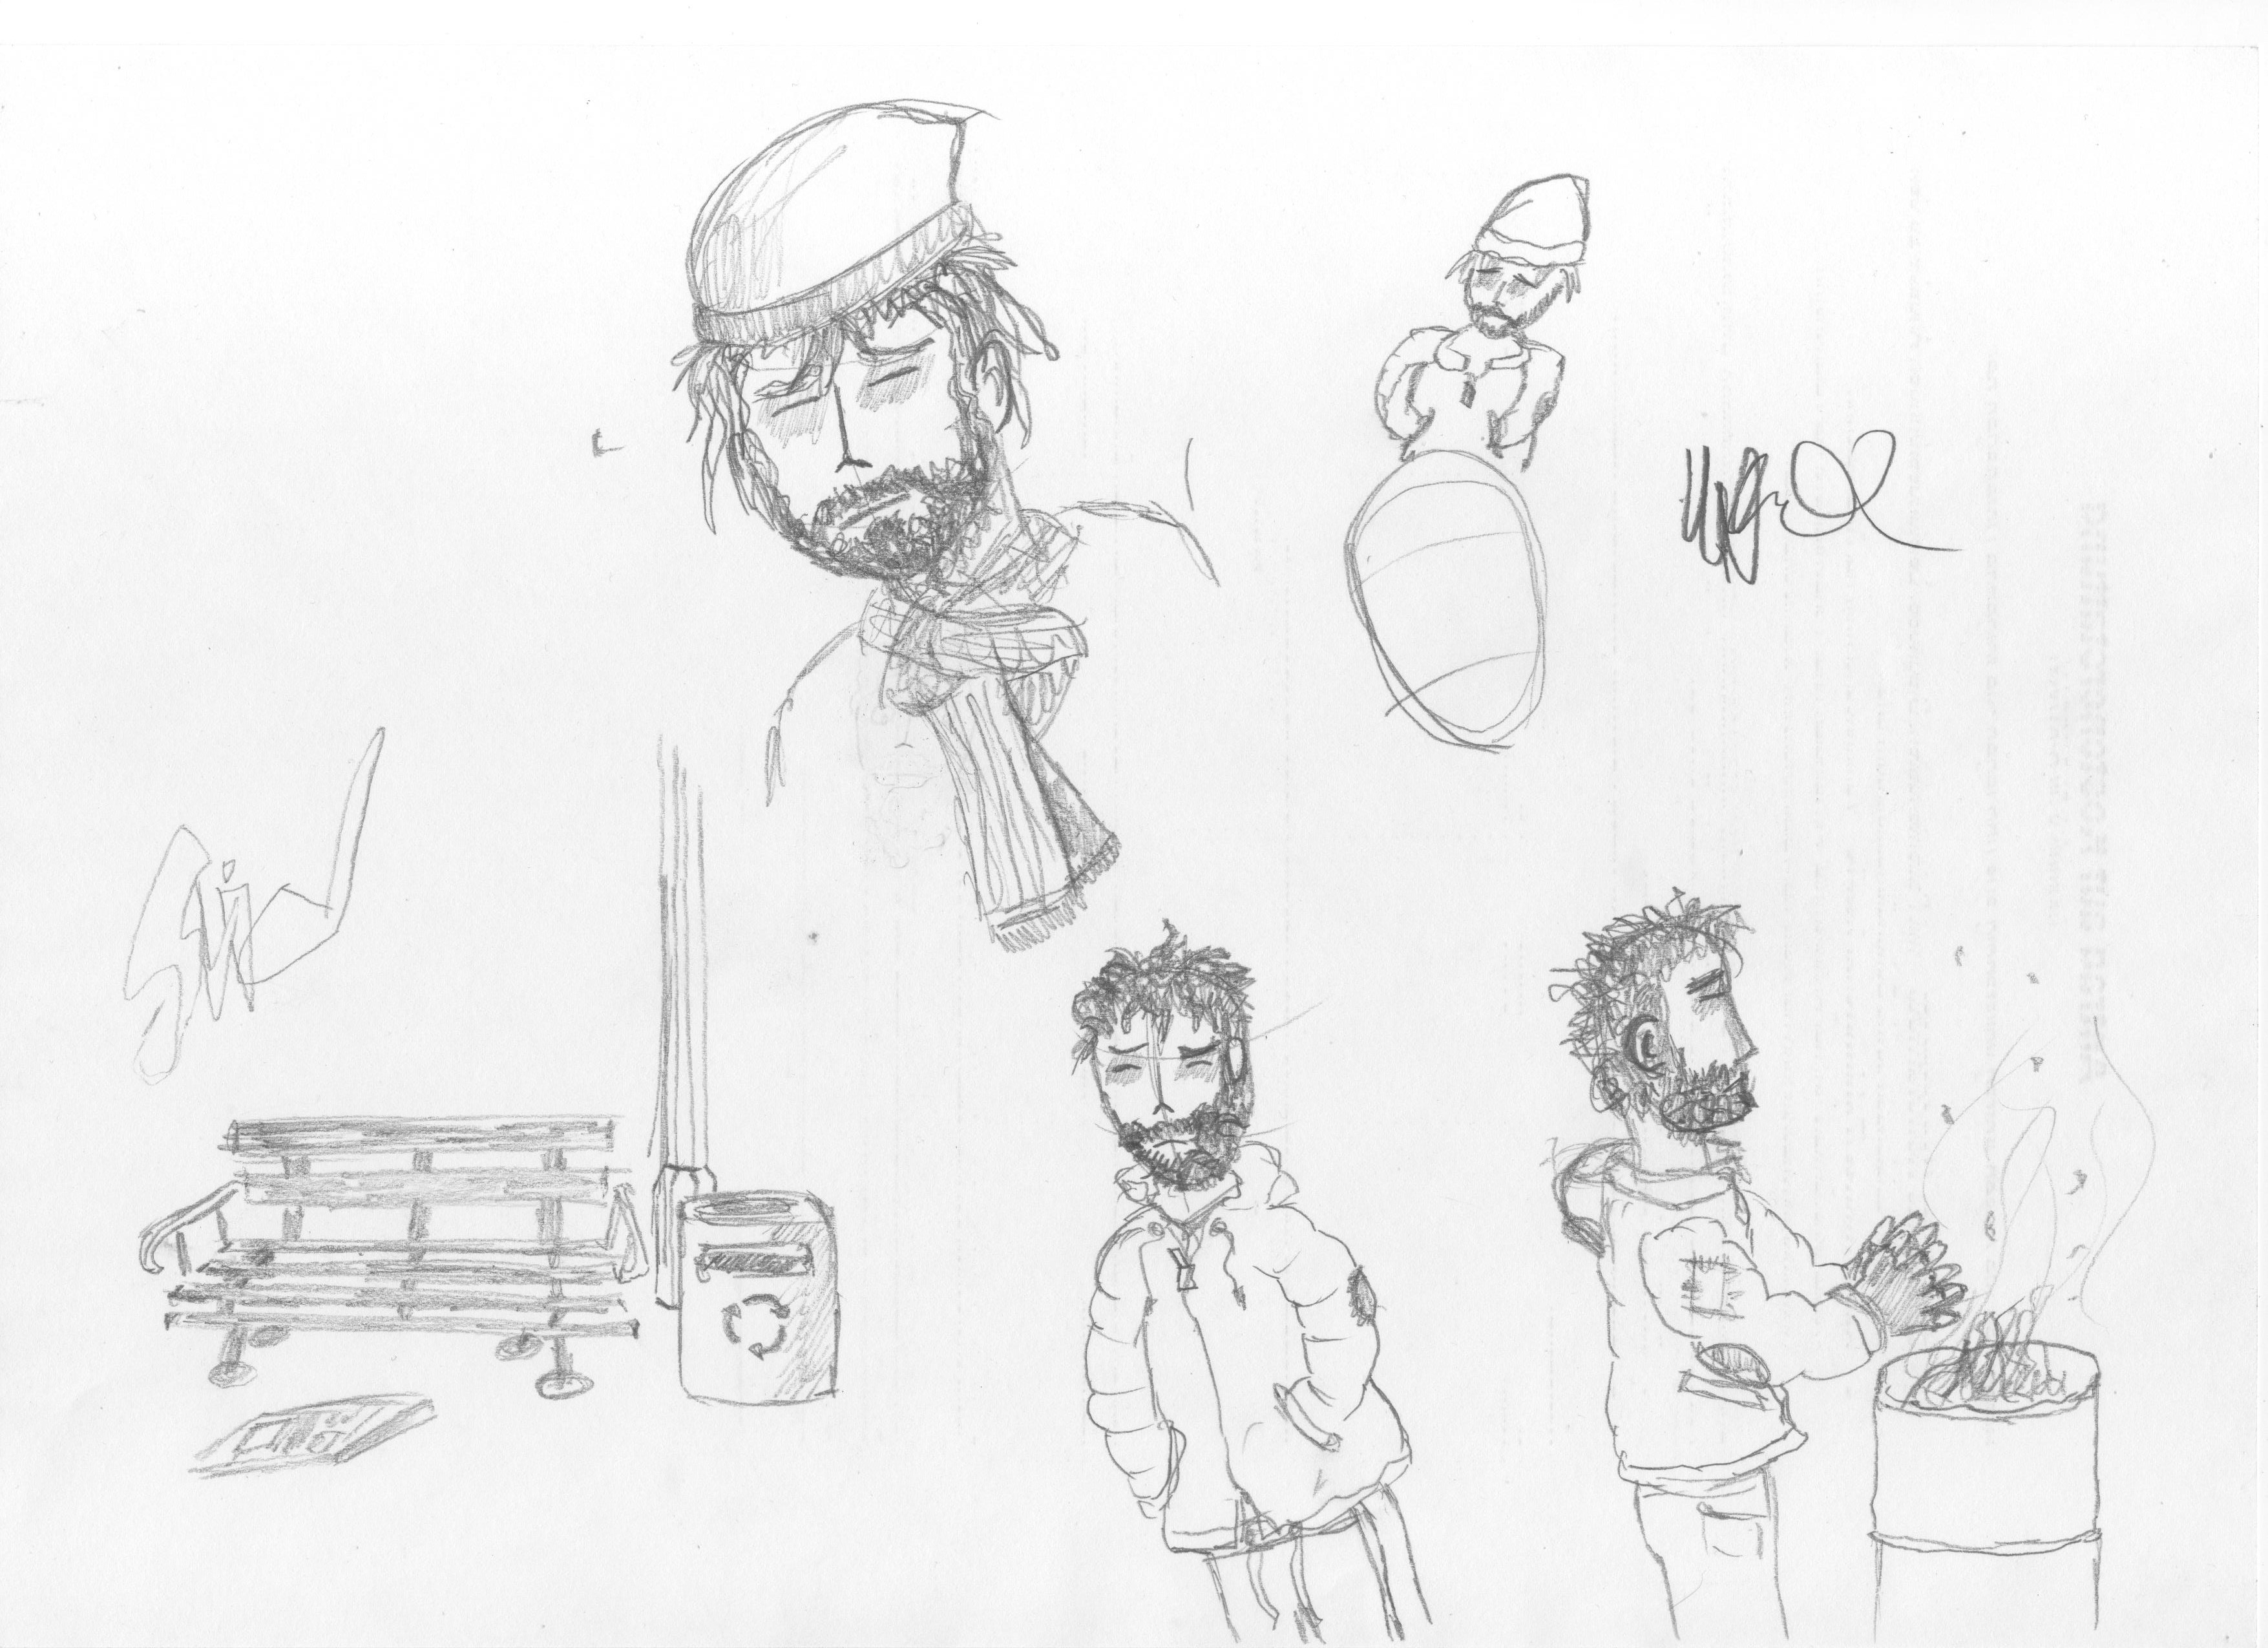
\includegraphics[width=1\textwidth]{concept1.jpg}
\caption{\label{fig:concept} Concept drawings}
\end{figure}

\pagebreak

\section{Forms of Engagement}
%thinking of Hunicke's 8 kinds of "fun" - what would you like to focus on?\\
%(1. Sensation - Game as sense-pleasure 
%2. Fantasy - Game as make-believe
%3. Narrative - Game as drama
%4. Challenge - Game as obstacle course
%5. Fellowship -  Game as social framework
%6. Discovery - Game as uncharted territory 
%7. Expression - Game as self-discovery 
%8. Submission - Game as pastime)\\
%\\
Based on Hunicke's 8 kinds of "fun" we will focus on:\\
\\
\textbf{Narrative} - Game as drama\\
The narrative of the game is a very big deal. We want to build a unique story for every player based on his decisions.\\ 
\\
\textbf{Challenge} - Game as obstacle course\\
As stated beforehand our game is very hard and at times it might even seem unfair. This contributes to the atmosphere we want the player to experience.\\
\\
\textbf{Discovery} - Game as uncharted territory\\
The player is able to go anywhere he wants to from the start of our game. This is actually a very important aspect. We want the player to discover places he or she might in hindsight would have loved to avoid.\\
\\
\textbf{Expression} - Game as self-discovery\\

% ______________________
% chapter Game Details
% ______________________


\chapter{Gameplay and Game Setting}

\section{Mood and Emotions}
We mainly want the player to experience a depressive and revealing game. We want the player to feel helpless for the most time, because we want him or her to feel almost ecstatic when improving his situation just a little bit. 

\section{Story}

On a cold, harsh winter morning, a nameless derelict wakes up and is confronted with a choice. "How will I hold up today?", they think. "Should I test my chances at the grocery? Maybe they'll have some scraps or left-overs. Or should I try welfare? Or beg? I need some money. Maybe Charles has a another job to offer. Even if we get caught, that would mean a warm night or two and some hot meals. Still it's always risky. Maybe the lads up-town have some change to spare. Ronnie got really lucky yesterday. Maybe he still has some left and I can borrow some. Or take it. He's anyway doing much better than I am. Though, can I run fast enough? Perhaps I should try my luck with the trash. I could get crafty and maybe sell something. That wouldn't even be begging.."

%the story of the game
%The story depends on the players choices, so everyone can get his own unique experience playing \textit{Homeless}.\\
%PLEASE EDIT: THESE ARE JUST SOME THOUGHTS\\
%Basically you start as a homeless guy or gal living on the street. You have neither money, nor food or a home. You try to get through the day by finding something to eat and a place to sleep. By traveling the world you find out how you even got to live on the streets. You will meet people you know from your past life, you will meet people from your present life and you will also meet people you don't know. Talking to them and being attentive while walking through the world will let you find out more about yourself...
%newspaper for data and time
\section{World/Environment} 
The game is set in an urban environment in a larger city.
%also, add here a map of your environment or a picture of your world if necessary

\section{Objects in the Game}
\begin{itemize}
	\item Different kinds of food
	\item Different kinds of medicine
	\item Money
	\item Other Stuff
\end{itemize}

\section{Characters in the Game}
\begin{itemize}
	\item You
	\item People from your past life
	\item People from your present life
	\item Others
\end{itemize}

\section{Main Objective}
Surviving.

\section{Core Mechanics}

\textbf{Social System}\\
This is more or less \textbf{the} core mechanic of the game. The Social-System in \textit{Homeless} keeps track of the players decisions and how they affect his or her reputation.\\
\\
\textbf{Job system}\\
You can take jobs in \textit{Homeless}. This doesn't mean that you simply go somewhere and get offered a desk job at a nice little firm. It means selling drugs, helping other homeless people, getting medicine for those who need it, beating up pedestrians or letting yourself get filmed when you are beat up by some teenage kids. Jobs can get you money, food, shelter or simply new friends, but will most likely affect a few of your stats.\\
\\
\textbf{Static World}\\
The first prototype of \textit{Homeless} includes a static world. We plan on expanding it dynamically as one of our next steps.\\
\\
\textbf{Interact with environmental objects}\\
You can interact with several objects like different kinds of food, benches, NPCs, tools, weapons, medicine etc.\\
\\
\textbf{Theft}\\
If you like it or not theft will most probably be inevitable to survive the winter.\\
\textit{Homeless} also includes a Pickpocket-System where you can pickpocket basically every other character you meet. Pickpocketing others will affect your reputation if you get caught and will therefore influence your further going.\\
\\
\textbf{Imprisonment}\\
Violence, Drugs or simply being at the wrong place at the wrong time. Actions have consequences and the consequence for living a rough life often means prison. If you have done something "bad", or at least something which isn't socially accepted, you will get jailed if caught by the police.\\
\\

\section{Controls}
The game is controlled via mouse. Clicking on objects and characters activates them or starts an interaction. Clicking on an empty spot on the level makes the main character move towards that point.

% ______________________
% chapter Front End
% ______________________


\chapter{Front End}
The game uses a simple front end, we want to show the player as little permanent information as possible on screen but rather have subtle hints during gameplay that tell them about their current situation. So there are no health or hunger displays or anything similar.

\section{Start Screen}
The start screen is simple, containing only the game title and 3 menu options to start a new game, continue the existing one or leave the game. Note how the options are purposely not named "New game" or "Quit game". The background of the start screen contains a scrolling view of the world.
\begin{figure}[h]
\centering
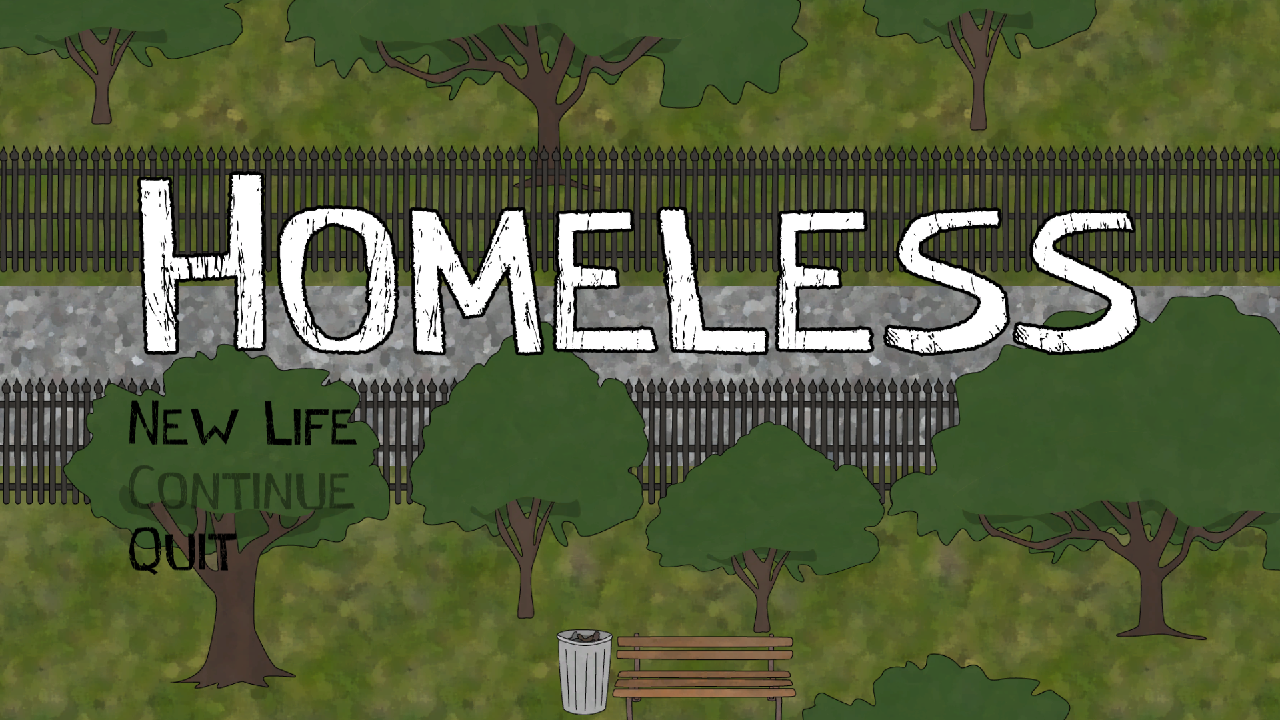
\includegraphics[width=0.8\textwidth]{main_screen.png}
\caption{\label{fig:start} Start screen}
\end{figure}

\section{Menus}
Following the principle of showing the user as little UI as possible, there will also be as little menus as possible. Players will choose options by clicking on the appropriate spot in the world rather than selecting things in a menu.

\pagebreak

\section{End Screen}
The end screen contains the simple "End" followed by a short description as to why the game ended, for example due to the player character dying.
\begin{figure}[h]
\centering
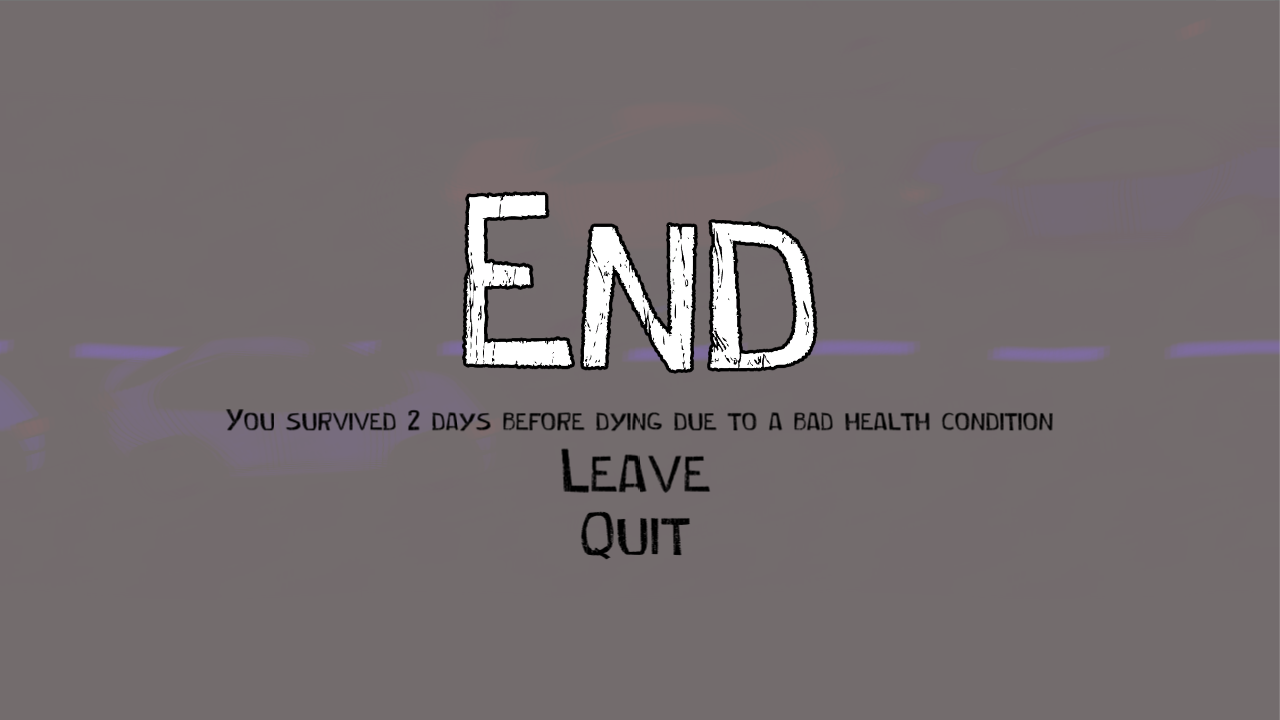
\includegraphics[width=0.8\textwidth]{end_screen.png}
\caption{\label{fig:end} End screen}
\end{figure}

% ______________________
% chapter Game Details
% ______________________


\chapter{Technology}

\section{Target Systems}
The game is designed for Desktop PC use, mainly Windows and Linux but Unity allows other export options so this is not set in stone.

\section{Hardware}
The game is controlled by mouse and keyboard.

\section{Development Systems/Tools}
%please describe the tools you are using (game engine, art tools, ..)
Unity is used to develop the game, as it is a simple engine that fulfills all our requirements in 3D and 2D. Task management is done via Trello and GitHub and Git is used for version control. 2D art is created with Illustrator and/or Photoshop and additionally Fireworks. Character animations are created in Spriter.

% ______________________
% chapter Game Details
% ______________________


\chapter{Topic and Inclusion }
\section{Main Theme}
\textit{Homeless} tells a story from a different perspective. 
We hope that by showing people how hard the life of a homeless person can be, it will be easier for them to sympathize with them.

% ______________________
% chapter Game Details
% ______________________


\chapter{Marketing and Publishing Strategy}
The game will be promoted using social media, mainly Twitter and YouTube. Twitter will be used for sharing news and updates about the game as well as making people aware of it. On YouTube we will share more in-depth progress updates and game feature videos.\\
The game will be published on \hyperlink{https://itch.io/}{itch.io} when it is finished.



% ______________________
% chapter Game Details
% ______________________


\chapter{Timeline}
\begin{table}[h]
\centering
\begin{tabular}{|c|l|c|}
\hline
Milestone & Description & Date \\\hline
1 & Fixate core game mechanics and submit design document  & 08.12 \\
2 & Create game skeleton & 22.12 \\
3 & Implement base mechanics and create provisional assets & 05.01 \\
4 & Finalise first prototype & 10.01 \\
S1 & Submit a working prototype & 12.01 \\
5 & Agree on final feature set & 01.02 \\
6 & Realise core gameplay mechanics & 10.02 \\
7 & Finalise implementation and assets & 02.03 \\
S2 & Submit final game and presentation & 09.03 \\
\hline
\end{tabular}
\caption{\label{tab:schedule}Tentative Project Timeline}
\end{table}


% ______________________
% chapter Game Details
% ______________________


\chapter{Team and Credits}

\section{Team}
\begin{itemize}
\item Project Management: Toller Maximilian
\item Game Assets: Gabl Sebastian
\item Programming: Huber Christian, Voulgaridis Anastasios
\item Game Design: Andrusyak Bohdan, Potzinger Dominic
\item Story Design: Huber Christian, Toller Maximilian
\end{itemize}

\section{Credits}
\begin{itemize}
\item \hyperlink{https://www.dafont.com/cordelina.font}{Cordelina} font by Samuel de Angelis
\item \hyperlink{https://github.com/loodakrawa/SpriterDotNet/tree/develop/SpriterDotNet.Unity}{SpriterDotNet} library by Luka "loodakrawa" Sverko
\item Game soundtrack by Michael Berr
\end{itemize}




%\bibliographystyle{alpha}
%\bibliography{sample}

\end{document}
